% Opcje klasy 'iithesis' opisane sa w komentarzach w pliku klasy. Za ich pomoca
% ustawia sie przede wszystkim jezyk i rodzaj (lic/inz/mgr) pracy, oraz czy na
% drugiej stronie pracy ma byc skladany wzor oswiadczenia o autorskim wykonaniu.\\
%\ifx\HCode\UnDef\else\hypersetup{tex4ht}\fi
\documentclass[declaration,shortabstract]{iithesis}
\usepackage{polski}
\usepackage[utf8]{inputenc}
\usepackage{listings}
\usepackage{graphicx}


%%%%% DANE DO STRONY TYTYŁOWEJ
% Niezaleznie od jezyka pracy wybranego w opcjach klasy, tytul i streszczenie
% pracy nalezy podac zarowno w jezyku polskim, jak i angielskim.
% Pamietaj o madrym (zgodnym z logicznym rozbiorem zdania oraz estetyka) recznym
% zlamaniu wierszy w temacie pracy, zwlaszcza tego w jezyku pracy. Uzyj do tego
% polecenia \fmlinebreak.
\polishtitle    {Analiza drzew samoorganizujących}
\englishtitle   {English title}
\polishabstract {W  tej pracy porównuje wydajność drzewa Splay, drzewa Tango oraz drzewa czerwono - czarnego}
\englishabstract{\ldots}
% w pracach wielu autorow nazwiska mozna oddzielic poleceniem \and
\author         {Julia Majkowska}
% w przypadku kilku promotorow, lub koniecznosci podania ich afiliacji, linie
% w ponizszym poleceniu mozna zlamac poleceniem \fmlinebreak
\advisor        {dr hab. Marcin Bieńkowski}
%\date          {}                     % Data zlozenia pracy
% Dane do oswiadczenia o autorskim wykonaniu
%\transcriptnum {}                     % Numer indeksu
%\advisorgen    {dr. Jana Kowalskiego} % Nazwisko promotora w dopelniaczu
%%%%%

%%%%% WLASNE DODATKOWE PAKIETY
%
%\usepackage{graphicx,listings,amsmath,amssymb,amsthm,amsfonts,tikz}
%
%%%%% WŁASNE DEFINICJE I POLECENIA
%
%\theoremstyle{definition} \newtheorem{definition}{Definition}[chapter]
%\theoremstyle{remark} \newtheorem{remark}[definition]{Observation}
%\theoremstyle{plain} \newtheorem{theorem}[definition]{Theorem}
%\theoremstyle{plain} \newtheorem{lemma}[definition]{Lemma}
%\renewcommand \qedsymbol {\ensuremath{\square}}
% ...
%%%%%

\begin{document}

%%%%% POCZĄTEK ZASADNICZEGO TEKSTU PRACY

  

\chapter{Wprowadzenie}  

\section{Wstęp}  

Binarne drzewo przeszukiwań to jedna z najbardziej podstawowych struktur danych w informatyce. Stosuje się je w wielu systemach informatycznych i algorytmach. Ideą struktury jest trzymanie elementów w wierzchołkach, trzymających wartość elementu oraz wskaźniki na lewe i prawe poddrzewo. Elementy umieszcza się w strukturze w taki sposób, aby wszystkie wartości elementów znajdujące się w lewym poddrzewie wierzchołka \(w\) były elementami mniejszymi od \(w\) w zdefiniowanym porządku. Analogicznie wszystkie elementy w prawym poddrzewie są elementy większe w tym porządku. Na tak uporządkowanych danych można wyszukiwać danej wartości \(v\) poprzez zagłębianie się w drzewo wybierając odpowiednio lewe lub prawe poddrzewo w zależności od wyniku porówna \(v\) z wartością korzenia. W najbardziej podstawowej formie tej struktury operacje wstawiania, wyszukiwania i usuwania wykonuje się w czasie O(H), gdzie H to wysokość drzewa. W pesymistycznym wypadku jest to czas liniowy od liczby elementów w strukturze. Złożoność operacji słownikowych na drzewie BST zależy od głębokości drzewa, dlatego powstało wiele struktur danych ograniczających maksymalną głębokość drzewa. Spośród deterministycznych można wymienić drzewa Splay, drzewa AA oraz czerwono-czarne, obsługujące operacje słownikowe w pesymistycznym czasie O(logn).  

 

\section{Problem optymalnego drzewa binarnego}  

W wielu zastosowaniach dane nie podlegają rozkładowi jednostajnemu tylko przejawiają jakąś lokalność. Przykładowo, jeśli dla drzewa 100- elementowego będą się pojawiać głównie zapytania o jeden element, można by znacząco zmniejszyć czas działania przesuwając dany element do korzenia. W takim wypadku struktura naszego drzewa zależy od zapytań. Problem znajdowania drzewa binarnego, które przy użyciu najmniejszej liczby operacji obsłuży ciąg zapytań to problem optymalnego drzewa binarnego. Możemy rozróżnić dwa warianty tego problemu statyczny oraz dynamiczny.  

\subsection{Statyczne optymalne drzewo binarne}  

Wg. definicji Knutha definiujemy uporządkowany ciąg elementów \(e_1...e_n\), ciąg prawdopodobieństw \(A_1...A_n\), będące prawdopodobieństwem wykonania wyszukiwania\(e_i\) i  \(B_0 … B_n\), będące prawdopodobieństwem wyszukania elementu z przedziału \([e_i, e_{i+1}]\). Szukamy drzewa minimalizujący oczekiwany czas wyszukiwania.  

Wraz z definicją problemu Knuth opublikował algorytm opierający się n a programowaniu dynamicznym, znajdujący optymalne drzewo binarne w czasie O(\(n^2\)). W 1975 r. Kurt Mehlhorn opublikował algorytm aproksymacyjny, działąjący w czasie O(n). Dla wariantu, w którym \(B_i = 0\), istnieje algorytm Garsia-Wachsa, który znajduje optymalne drzewo w czasie O(nlogn).  

\subsection{Dynamiczne optymalne drzewo binarne}  

W dynamicznym wariancie problemu mamy na wejściu ciąg zapytań \(x_i\) o wyszukanie klucza \(k \in [1, n]\). Dla każdego zapytania o wartość \(w\) zaczynamy ze wskaźnikiem na korzeń drzewa i wykonując tylko niżej wymienione operacje chcemy przesunąć wskaźnik na wierzchołek zawierający klucz o wartości \(w\). Dozwolone operacje to:  

\begin{enumerate}  

\item {Przesunąć wskaźnik na lewego syna obecnie wskazanego wierzchołka}  

\item {Przesunąć wskaźnik na prawego syna obecnie wskazanego wierzchołka}  

\item {Przesunąć wskaźnik na rodzica obecnie wskazanego wierzchołka}  

\item {Wykonać pojedynczą rotację obecnie wskazywanego wierzchołka. Poniżej ilustracja pojedynczej rotacji punku x w prawo}   

\end{enumerate}   

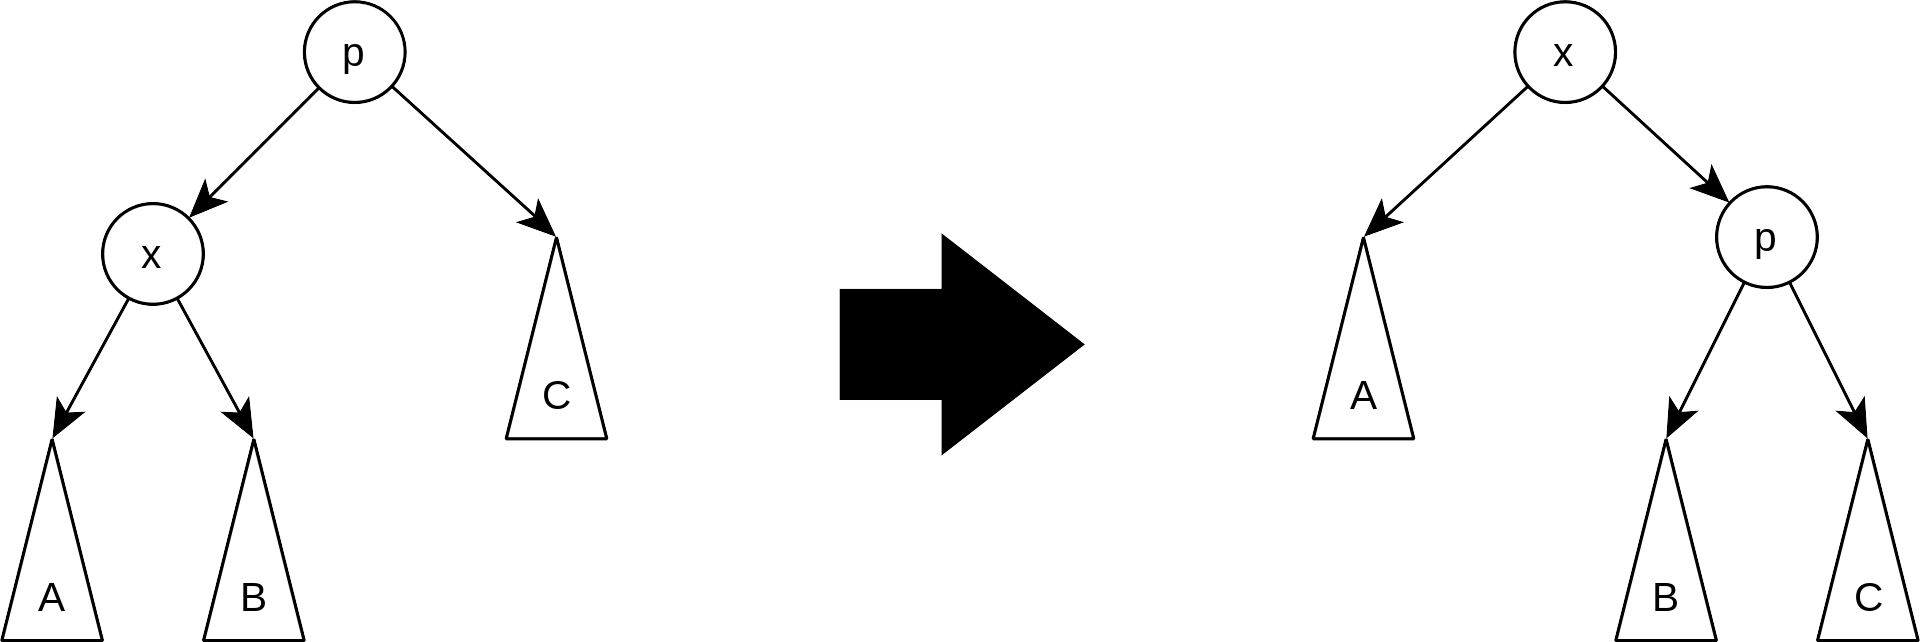
\includegraphics[scale = 0.75]{Splay_tree_zig.png}

W tym problemie wyszukujemy drzewo, które minimalizuje liczbę operacji koniecznych do obsłużenia ciągu zapytań \(x_i\).  

Dla każdego ciągu zapytań istnieje minimalny ciąg operacji odpowiadający na te zapytania. Znalezienie takiego rozwiązania wymaga znajomości całego ciągu zapytań z góry, co w wielu sytuacjach nie jest możliwe. Niech OPT(\(x_i\)) będzie minimalną liczbą operacji konieczna do zrealizowania ciągu zapytań \(x_i\), będziemy mówić, że drzewo jest dynamicznie optymalne, jeśli dla każdego ciągu wejść \(y_i\) algorytm wykonuje O(OPT(\(y_i\)) operacji. Innymi słowy ma stały współczynnik konkurencyjności. Udowodnienie dynamicznej optymalności dowolnego drzewa jest problemem otwartym.  

 

\chapter{Drzewa Splay}  

\section{Opis struktury} 

Drzewo Splay jest drzewem samoorganizującym się. Podstawią działania tej struktury jest operacja splay, polegająca na przesunięciu odpowiedniego wierzchołka do korzenia, korzystając z rotacji.  

\subsection{Splay} 

Operacja splay dla danego wierzchołka odbywa się w krokach, do momentu, kiedy wierzchołek nie stanie się korzeniem. Możemy wyróżnić 3 przypadki kroków operacji splay: 
\begin{enumerate} 

\item{ZIG - jeśli x jest synem korzenia wykonujemy pojedynczą rotację w stronę korzenia} 

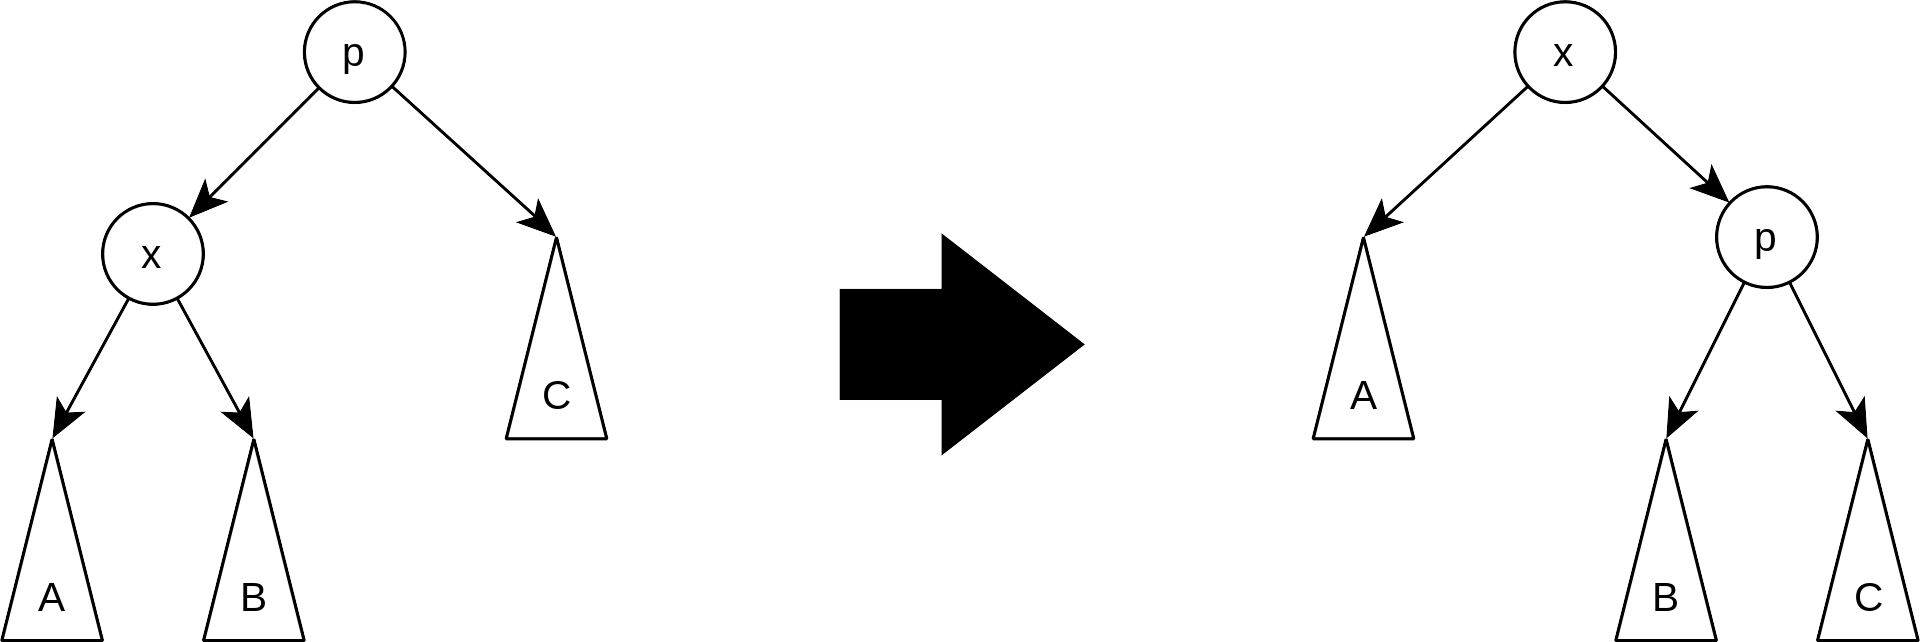
\includegraphics[scale = 0.75]{Splay_tree_zig.png}

\item{ZIGZIG - jeśli zarówno x i jego ojciec są lewymi synami wykonujemy u ojca rotację w prawo, a następnie rotujemy w prawo x. Analogicznie postępujemy kiedy x i jego ojciec są prawymi synami.} 

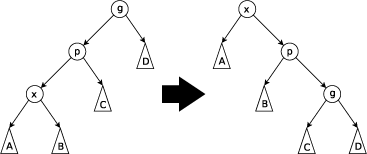
\includegraphics[scale=0.75]{Zigzig.png}
\item{ZIGZAG - jeśli x jest prawym synem, a jego ojciec jest lewym synem, rotujemy x w lewo a następnie w prawo. Analogicznie postępujemy kiedy x  jest lewym synem, a jego ojciec jest lewym synem.} 

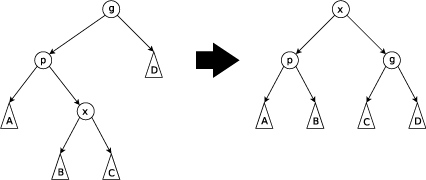
\includegraphics[scale=0.75]{Zigzag.png}
\end{enumerate}  

\begin{lstlisting} 

template<class T> 

void tree_vert<T>::splay(){ 

    while(!this-> is_root()){  

        if(this-> is_left()){ 
            if(this-> father-> is_root()){ 
                this->rotate_right(); 
                continue;  
            } 
            if(this->father-> is_left()){
                this->father->rotate_right(); 
                this->rotate_right(); 
            } 
            else{
                this->rotate_right(); 
                this->rotate_left(); 
            } 
        } 
        else{ 
            if(this-> father-> is_root()){ 
                this->rotate_left();     
                continue;  
            } 
            if(this->father-> is_left()){ 
                this->rotate_left(); 
                this->rotate_right(); 
            } 

            else{
                this->father->rotate_left(); 
                this->rotate_left(); 
            }  
        } 
    } 
} 

\end{lstlisting}  

\subsection{Wyszukiwanie}
Drzewo splay spełnia zależność BST, więc można wyszukiwać w nim elementu jak w normalnym drzewnie BST. Po wykonaniu znalezieniu odpowiedniego wierzchołka wykonujemy na nim operację splay przenosząc go do korzenia. 

\subsection{Rozdzielanie drzewa względem elementu}
Aby rozdzielić drzewo wględem danego elementu \(e\), wyszukujemy go w drzewie i wykonujemy operację splay na elemencie, na którym zakończyliśmy poszukiwanie. Wynikiem będą lewe i prawe poddrzewo korzenia. 

\subsection{Łączenie dwóch drzew}
Będziemy łaczyć drzewa o własności, że wszystkie elementy jednego drzewa są mniejsze od wszystkich elementów drugiego drzewa. Aby to zrobić wykonujemy operację splay na wierzchołku zawierającym minimalny element drugiego drzewa. Następnie podłączamy pierwsze drzewo jako lewe poddrzewo. 

\subsection{Wstawianie}
Aby wstawić element \(e\) do drzewa najpierw wyszukujemy go w drzewie, jeśli element już znajduje się w drzewie to wykonujemy operację splay na odpowiadającym mu wierzchołku. Jeśli elementu nie ma w drzewie, wtedy rozdzielamy drzewo względem \(e\) na drzewa \(d_1\) i \( d_2\). Następnie podłączamy \(d_1\) jako lewe poddrzewo elementu  \(e\) a \(d_2\) jako prawe poddrzewo. 

\subsection{Usuwanie}
Aby usunąć element, wyszukujemy go w drzewie i wykonujemy na odpowiadającym wierzchołku operację splay. Następnie łączymy lewę i prawe poddrzewo w jedno drzewo. 

\section{Złożoność}
\begin{tabular}{|c|c|c|}
\hline
Element algorytmu & Złożoność oczekiwana &  Złożoność pesymistyczna  \\
\hline
Pamięć & O(n) & O(n)  \\
\hline
Wstawianie & O(logn) & zamortyzowane O(logn)  \\
\hline
Usuwanie & O(logn) & zamortyzowane O(logn)  \\
\hline
Wyszukiwanie & O(logn) & zamortyzowane O(logn) \\
\hline

\end{tabular}

\chapter{ Drzewo Tango}


%%%%% BIBLIOGRAFIA

%\begin{thebibliography}{1}
%\bibitem{example} \ldots
%\end{thebibliography}

\end{document}